\chapter{Results}

%Results. Describe your results in a logical order: this may not necessarily be the order in which you did the experiments. Briefly summarise the main results at the end of each main experiment or sequence of associated experiments. Do not duplicate results -- put a table or a graph but not both unless the two methods of presentation demonstrate different points of importance. You must refer appropriately to figures or tables in the text and remember to emphasise and perhaps quote significant results. In particular, think about:

%o What were the results of your hypothesis tests, in the order you describe them in the Methods?
{\texorpdfstring
%TTo verify the fitting procedure for each of the three models (Classic, Depth, Perimeter) I created three different model simulations. I ran the simulation data through three NLLS fitting scripts to retrieve the known parameters ($\theta$, as calculated from \textit{nu} and metacommunity size \textit{J*K}, \textit{m\textsubscript{0}} and \textit{K}). Here I have plotted the know parameters against those estimated by the model fitting procedure. Once the model fitting procedures are validated, I use them to fit the three models to my datasets, as well as calculating critical area (\textit{A\textsubscript{crit}}) between niche-structured regime and colonisation-extinction regime. Using critical area estimates I test the hypothesis that regime change will occur at lower areas for more motile species and less isolated habitats. 

\section\section{Simulation}

\begin{figure}[htbp]
\centering
\subfloat[The Classic Model]{\label{fig:a}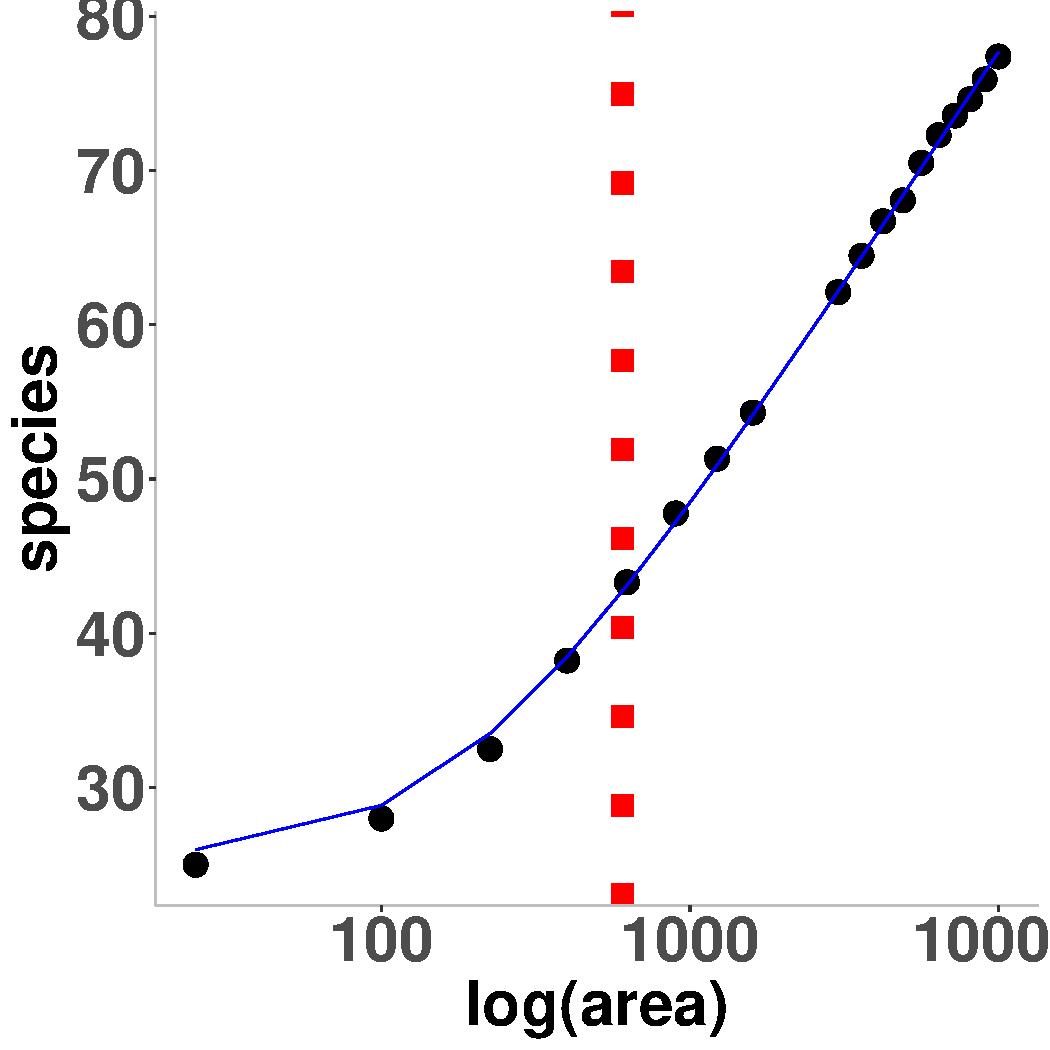
\includegraphics[width=0.3\linewidth]{../Results/Simulation/NLLSPlotClassic5.pdf}}
\subfloat[The Depth Model]{\label{fig:b}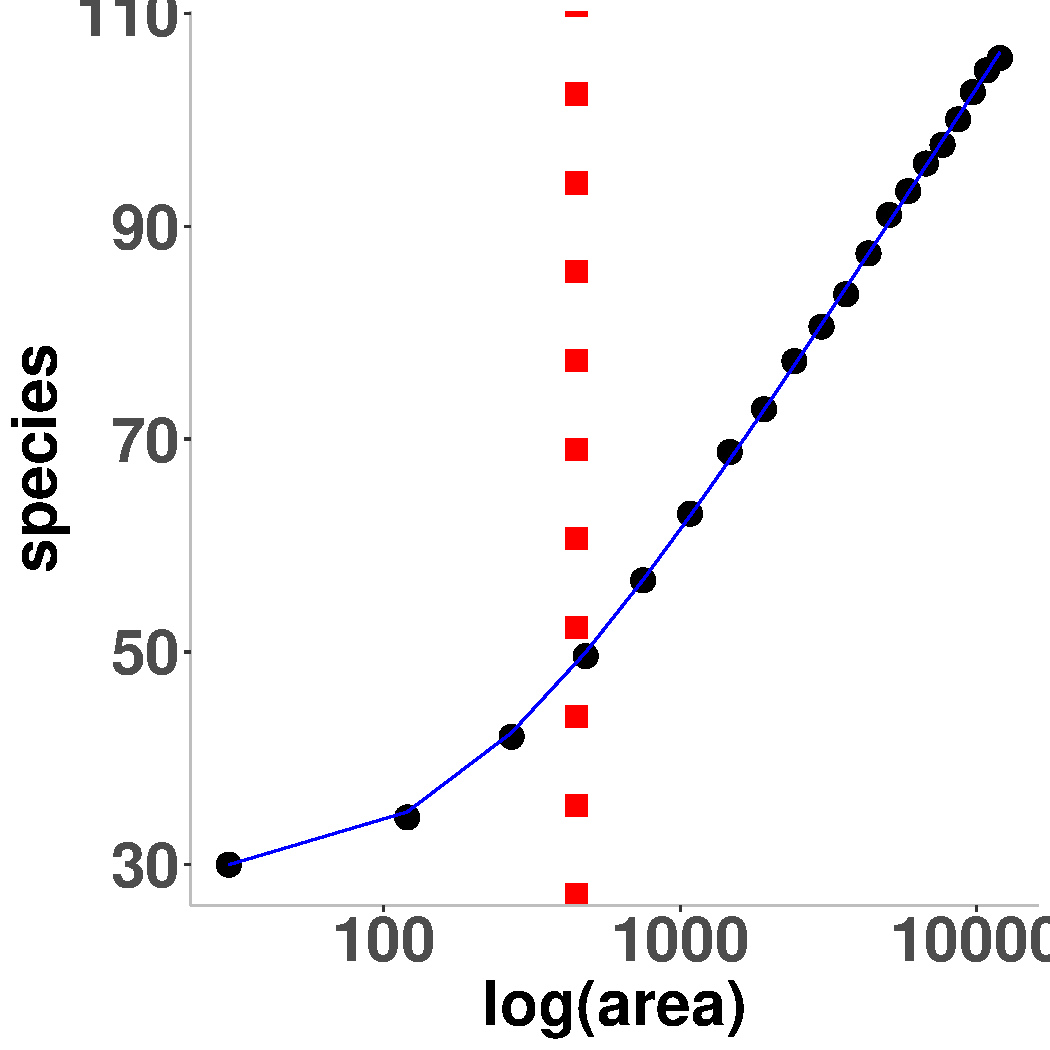
\includegraphics[width=0.3\linewidth]{../Results/Simulation/NLLSPlotDepth6.pdf}}
\subfloat[The Perimeter Model]{\label{fig:c}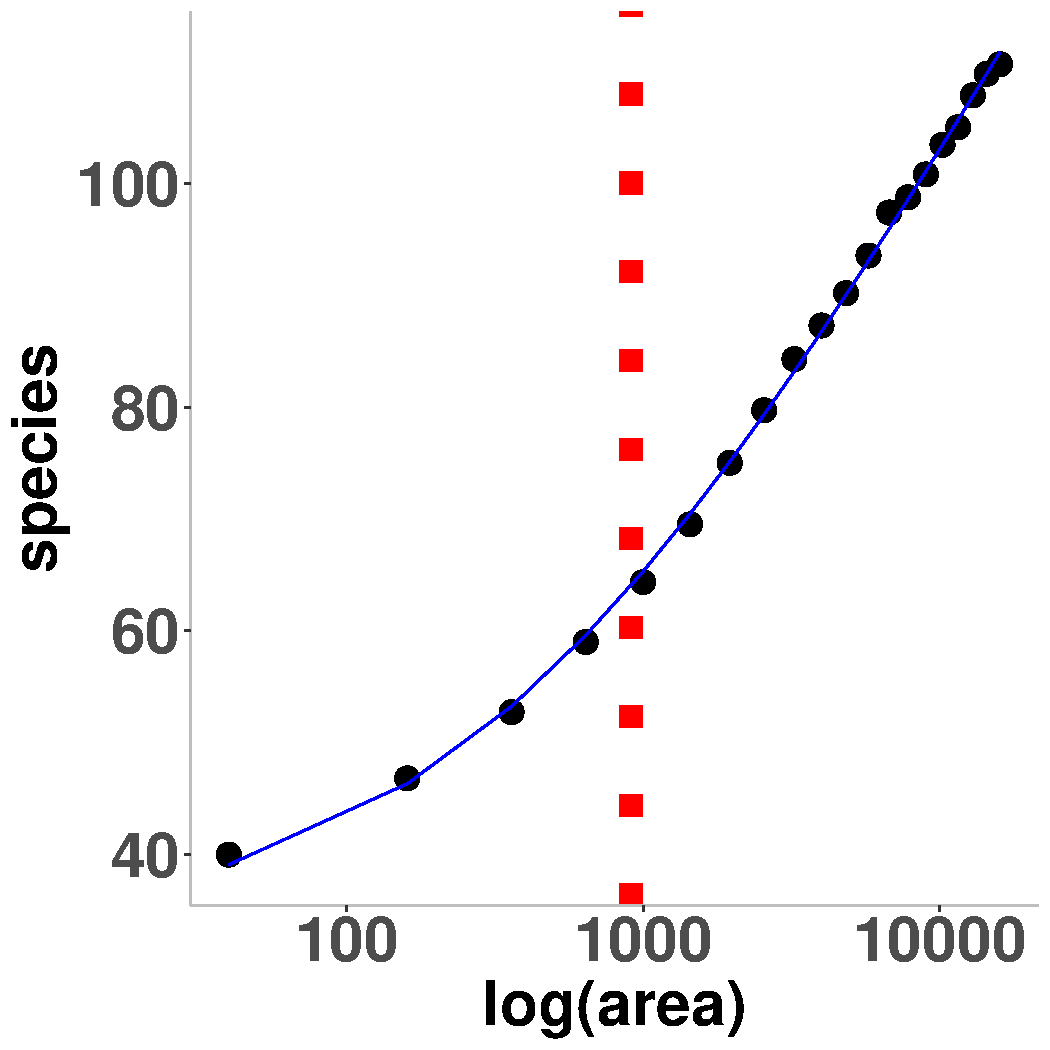
\includegraphics[width=0.3\textwidth]{../Results/Simulation/NLLSPlotPeri8.pdf}}
\bigskip 


Simulation data point \tikz\draw[black,fill=black] (0,0) circle (.5ex); \;\;NLLS fit \textcolor{blue}{\rule{1.5cm}{1mm}} \textit{A\textsubscript{crit}}\;\; \textcolor{red}{\rule{0.1cm}{1mm}}\; \textcolor{red}{\rule{0.1cm}{1mm}}\; \textcolor{red}{\rule{0.1cm}{1mm}}\; \textcolor{red}{\rule{0.1cm}{1mm}}\\

\caption{NLLS fitting of simulation data. A) The Classic Model with true parameters $\theta$=13, \textit{m\textsubscript{0}}=0.05, \textit{K}=25 and estimated parameters $\theta$=13, \textit{m\textsubscript{0}}=0.05, \textit{K}=25. B) The Depth Model with true parameters $\theta$=18, \textit{m\textsubscript{0}}=0.06, \textit{K}=30 and estimated parameters $\theta$=19, \textit{m\textsubscript{0}}=0.05, \textit{K}=30. C) The Perimeters Model with true parameters $\theta$=32, \textit{m\textsubscript{0}}=0.7, \textit{K}=40 and estimated parameters $\theta$=35, \textit{m\textsubscript{0}}=0.6, \textit{K}=39.}
\label{fig:myfig}
\end{figure}

\noindent My results verified that the simulation and analytic formula are in agreement as expected. The three \textit{A\textsubscript{crit}} formulas for each of the three model variations give reasonable estimations.

\subsection{Classic Model}

\noindent The Classic Model fitted the simulated data well. Estimated parameters were slightly higher than the true parameters for $\theta$ and slightly lower for \textit{m\textsubscript{0}} and \textit{K}. There was a significant difference between the true and estimated parameters for $\theta$ (p=0.0009, 9 df) and \textit{m\textsubscript{0}} (p=0.0002, 9 df). There was no significant difference in parameters for \textit{K} (p=0.08, 9 df).  As \textit{K} parameters showed no significant difference, and there was only a small difference between \textit{m\textsubscript{0}} and $\theta$ parameters, the model fitting process is considered validated and fit for applying to empirical datasets.   \\

\begin{figure}[htbp]
\centering
\subfloat[$\theta$ values]{\label{fig:a}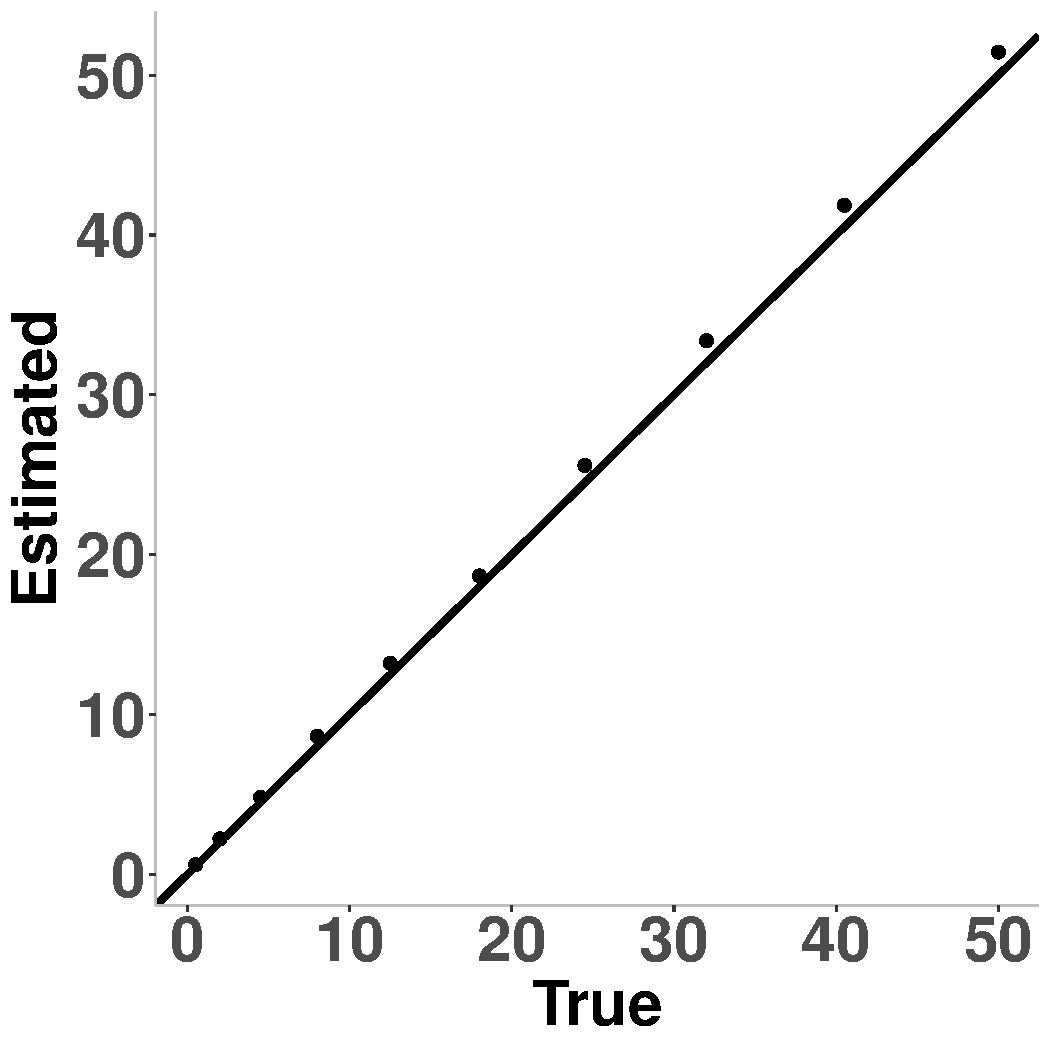
\includegraphics[width=0.3\linewidth]{AreaThetaResults.pdf}}
\subfloat[\textit{m\textsubscript{0}} values]{\label{fig:b}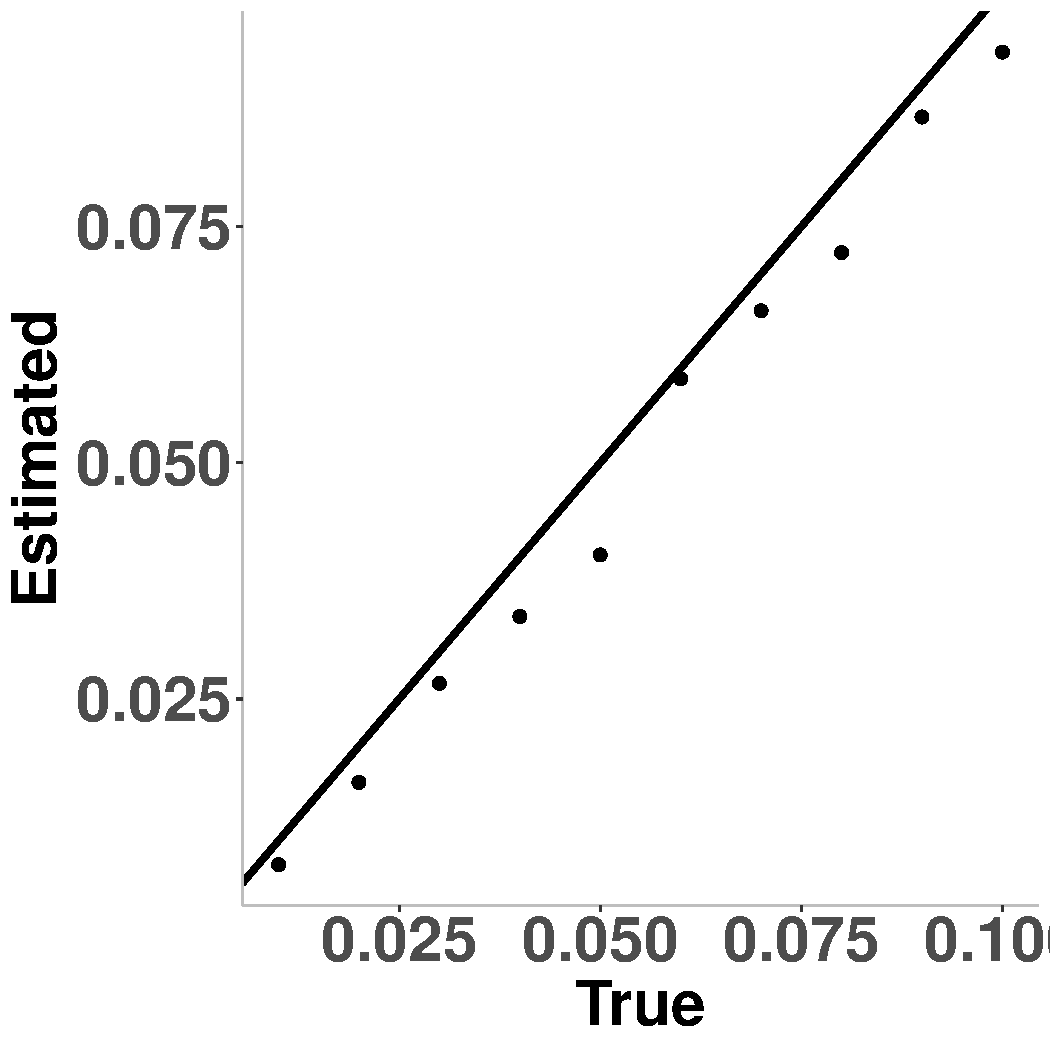
\includegraphics[width=0.3\linewidth]{Aream0Results.pdf}}
\subfloat[\textit{K} values]{\label{fig:c}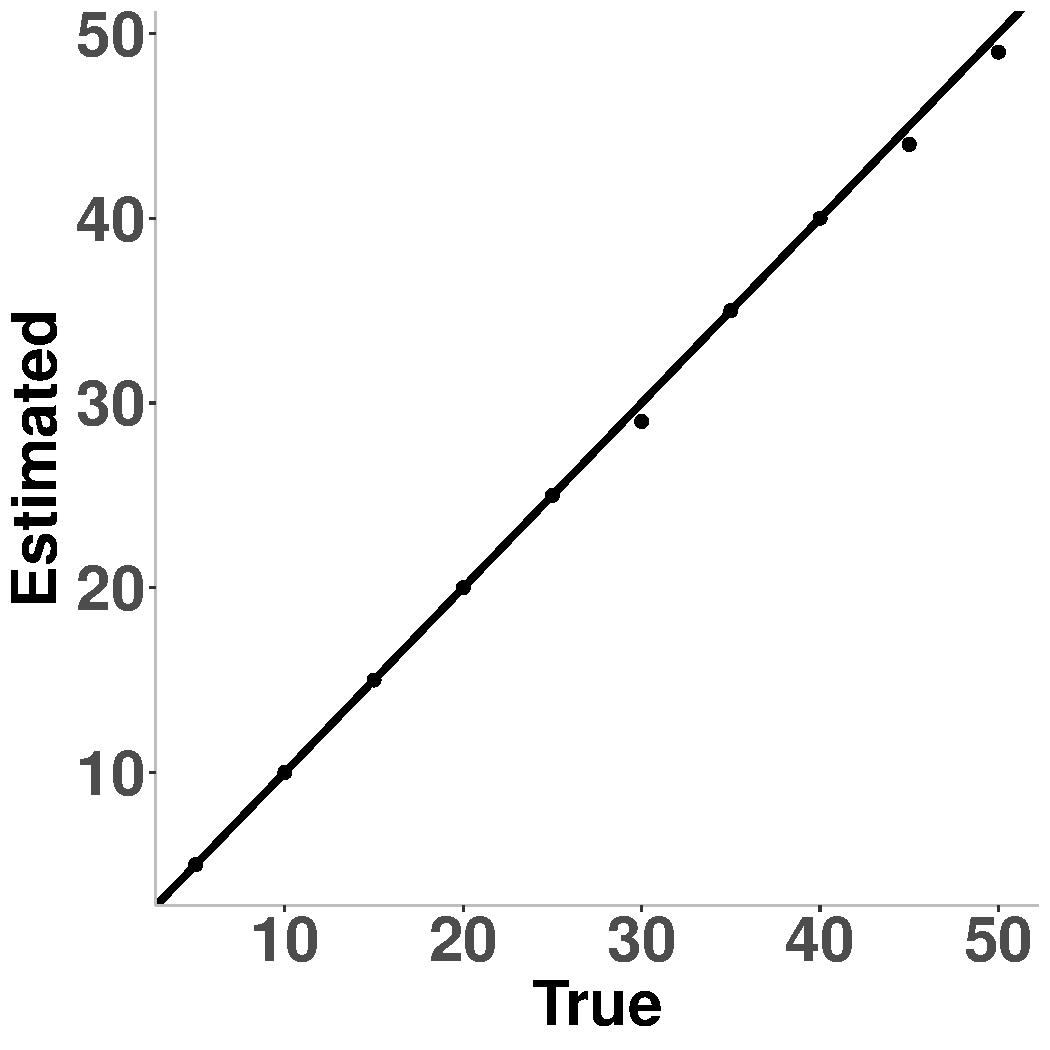
\includegraphics[width=0.3\textwidth]{AreaKResults.pdf}}
\bigskip

Parameter differences data point \tikz\draw[black,fill=black] (0,0) circle (.5ex); \;\; 1:1 line \textcolor{black}{\rule{1.5cm}{1mm}}\\

\caption{The true parameters values of $\theta$ (A), \textit{m\textsubscript{0}} (B) and \textit{K} (C) were simulated and the results fitted using the Classic Model analytical NLLS fitting procedure to get the parameters back. True and estimated values for the three fitted parameters are plotted above. Fittings of the Classic Model to simulated data returned mean R\textsuperscript{2} = 0.99, adjusted R\textsuperscript{2} = 0.99.}
\label{fig:myfig}
\end{figure}

\begin{table}[h!]
  \begin{center}
    \caption{Comparison between true and estimated mean parameters across 200 Classic Model simulations clustered into 10 groups where parameter values ($\theta$, \textit{m\textsubscript{0}}, \textit{K}) were the same for each simulation group with varying areas.}
    \label{table5}
    \pgfplotstabletypeset[
      multicolumn names, % allows to have multicolumn names
      col sep=comma, % the seperator in our .csv file
      display columns/0/.style={
		column name=$Parameter$, % name of first column
		string type},  % use siunitx for formatting
      display columns/1/.style={
		column name=$True$,
		column type={S},string type},
      display columns/2/.style={
		column name=$Estimated$,
		column type={S},string type},
      display columns/3/.style={
		column name=$Difference$,
		column type={S},string type},
           every head row/.style={
		before row={\toprule}, % have a rule at top
		after row={
			%\si{\ampere} & \si{\volt}\\ % the units seperated by &
			\midrule} % rule under units
			},
		every last row/.style={after row=\bottomrule}, % rule at bottom
    ]{ClassicParam.csv} % filename/path to file
  \end{center}
\end{table}



\subsection{Depth Model}

\noindent The Depth Model fitted the simulated data well. Estimated values of $\theta$ were higher, \textit{K} and \textit{m\textsubscript{0}} values were lower than the true parameters (Table 3.2). There was a significant difference between the true and estimated values for $\theta$ (p=0.0005, 9 df) and \textit{m\textsubscript{0}} (p=0.005, 9 df), but there was no significant difference for \textit{K} (p=0.168, 9 df). As \textit{K} showed no significant difference, and the difference in estimated $\theta$ and \textit{m\textsubscript{0}} values were low, the model fitting process is considered validated and fit for applying to empirical datasets.  

\begin{figure}[htbp]
\centering
\subfloat[$\theta$ values]{\label{fig:a}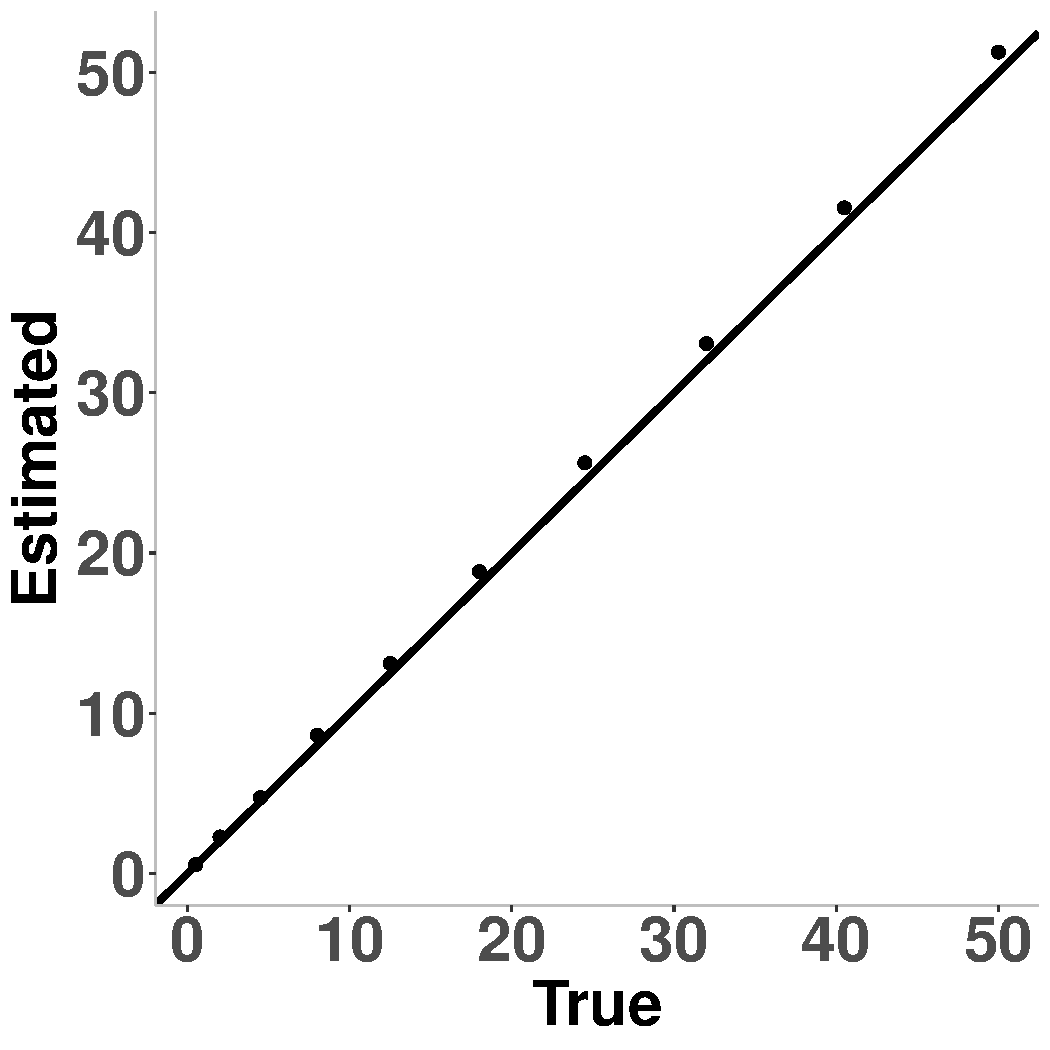
\includegraphics[width=0.3\linewidth]{DepthThetaResults.pdf}}
\subfloat[\textit{m\textsubscript{0}} values]{\label{fig:b}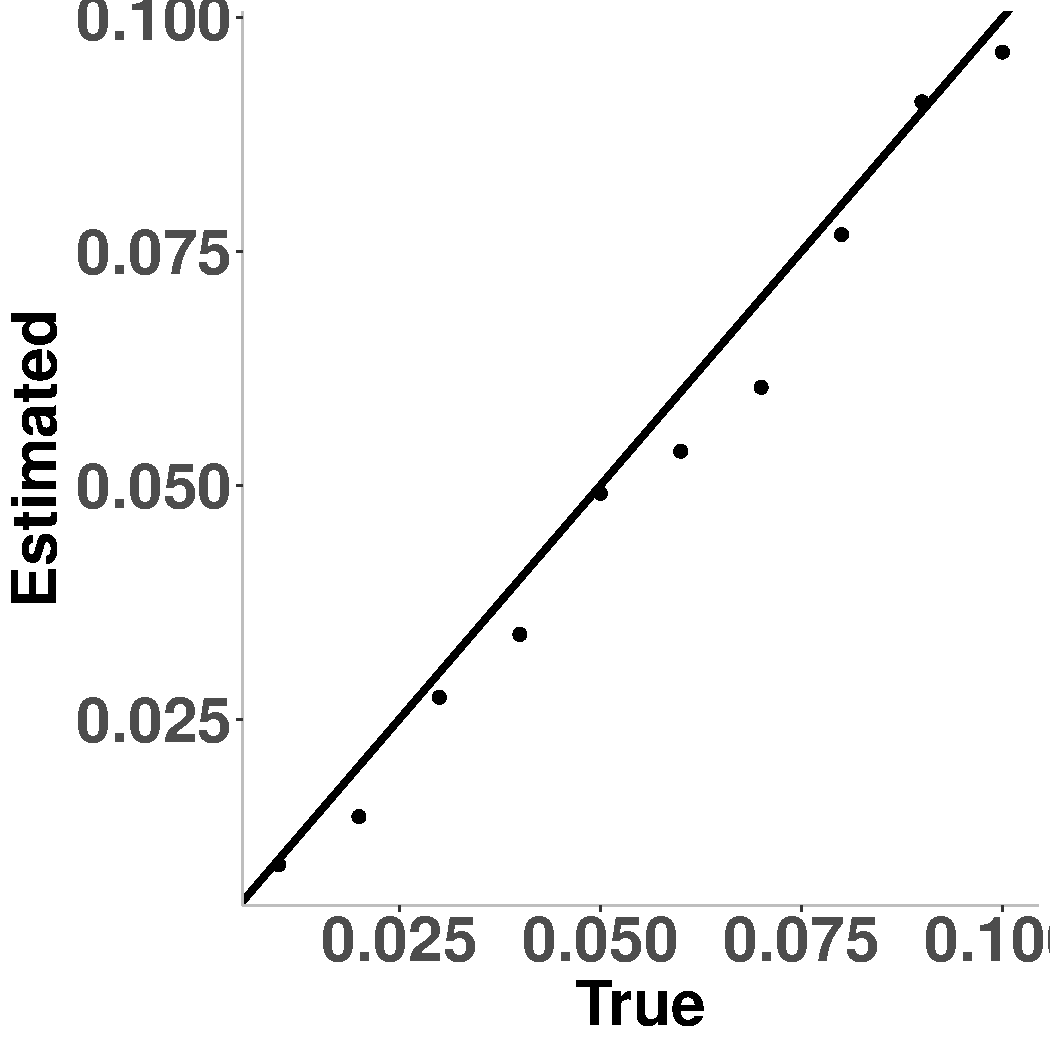
\includegraphics[width=0.3\linewidth]{Depthm0Results.pdf}}
\subfloat[\textit{K} values]{\label{fig:c}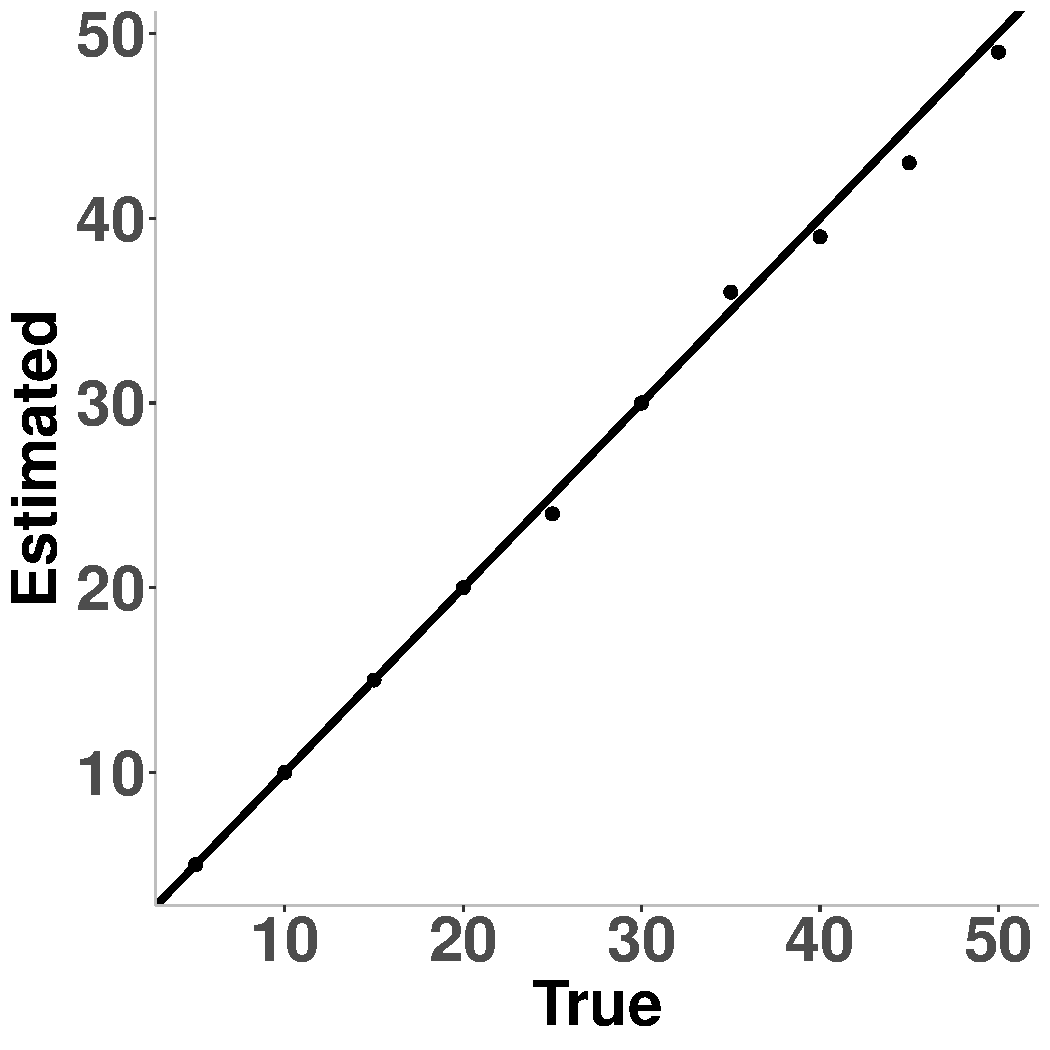
\includegraphics[width=0.3\textwidth]{DepthKResults.pdf}}
\bigskip

Parameter differences data point \tikz\draw[black,fill=black] (0,0) circle (.5ex); \;\; 1:1 line \textcolor{black}{\rule{1.5cm}{1mm}}\\

\caption{The true parameters values of $\theta$ (A), \textit{m\textsubscript{0}} (B) and \textit{K} (C) were simulated and the results fitted using the Depth Model analytical NLLS fitting procedure to get the parameters back. True and estimated values for the three fitted parameters are plotted above. Fittings of the Depth Model to simulated data returned mean R\textsuperscript{2} = 0.99, adjusted R\textsuperscript{2} = 0.99.}
\label{fig:myfig}
\end{figure}

\begin{table}[h!]
  \begin{center}
    \caption{Comparison between true and estimated mean parameters across 200 Depth Model simulations clustered into 10 groups where parameter values ($\theta$, \textit{m\textsubscript{0}}, \textit{K}) were the same for each simulation group with varying areas.}
    \label{table5}
    \pgfplotstabletypeset[
      multicolumn names, % allows to have multicolumn names
      col sep=comma, % the seperator in our .csv file
      display columns/0/.style={
		column name=$Parameter$, % name of first column
		string type},  % use siunitx for formatting
      display columns/1/.style={
		column name=$True$,
		column type={S},string type},
      display columns/2/.style={
		column name=$Estimated$,
		column type={S},string type},
      display columns/3/.style={
		column name=$Difference$,
		column type={S},string type},
           every head row/.style={
		before row={\toprule}, % have a rule at top
		after row={
			%\si{\ampere} & \si{\volt}\\ % the units seperated by &
			\midrule} % rule under units
			},
		every last row/.style={after row=\bottomrule}, % rule at bottom
    ]{DepthParam.csv} % filename/path to file
  \end{center}
\end{table} 


\subsection{Perimeter Model}


\begin{figure}[htbp]
\centering
\subfloat[$\theta$ values]{\label{fig:a}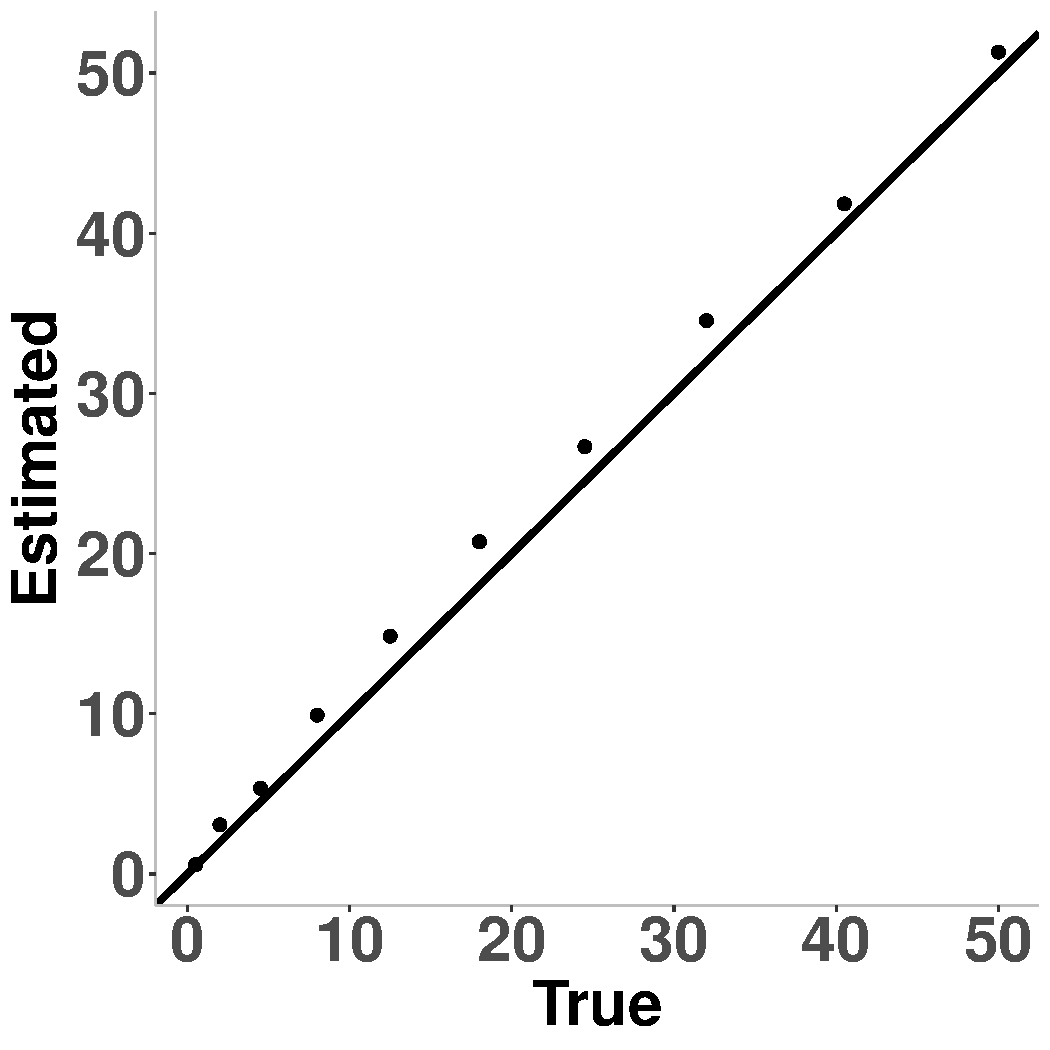
\includegraphics[width=0.3\linewidth]{PeriThetaResults.pdf}}
\subfloat[\textit{m\textsubscript{0}} values]{\label{fig:b}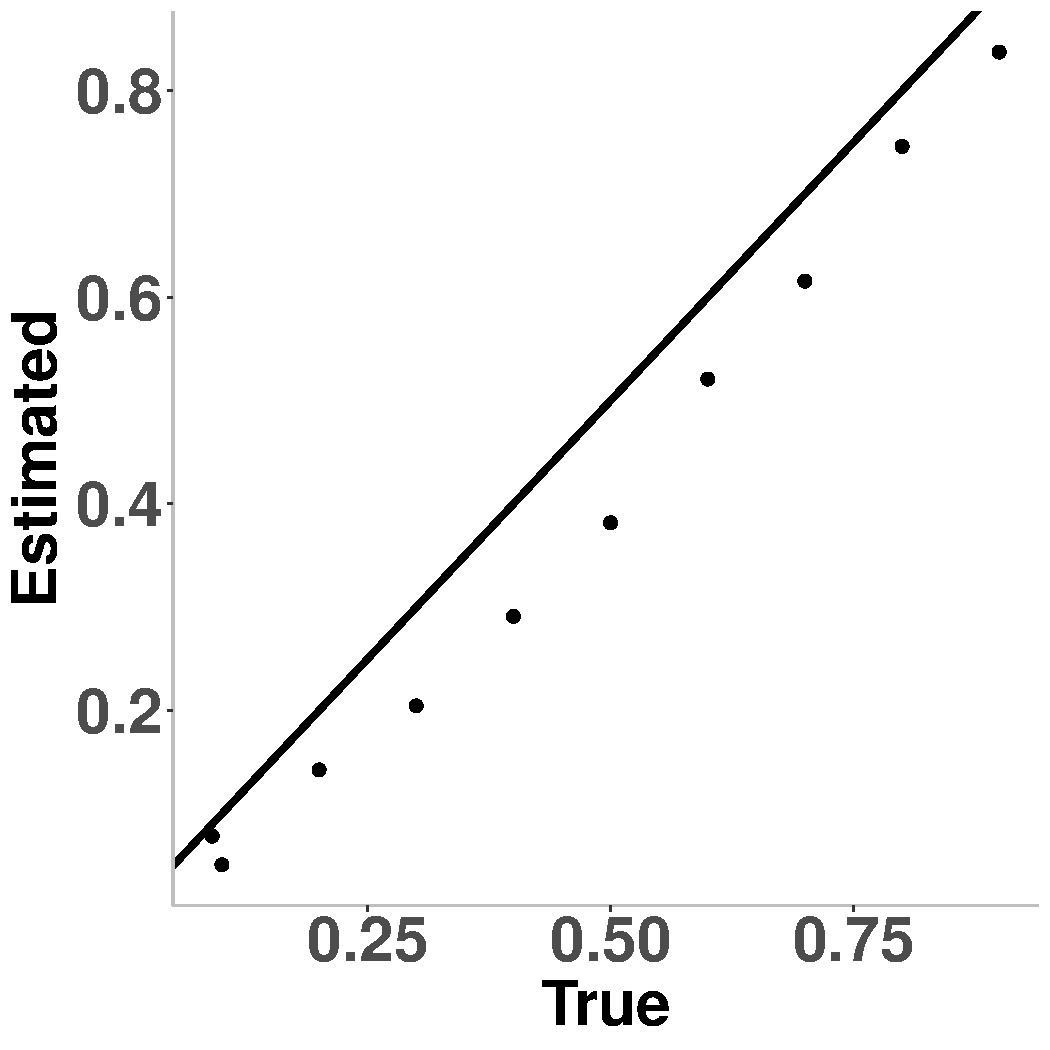
\includegraphics[width=0.3\linewidth]{Perim0Results.pdf}}
\subfloat[\textit{K} values]{\label{fig:c}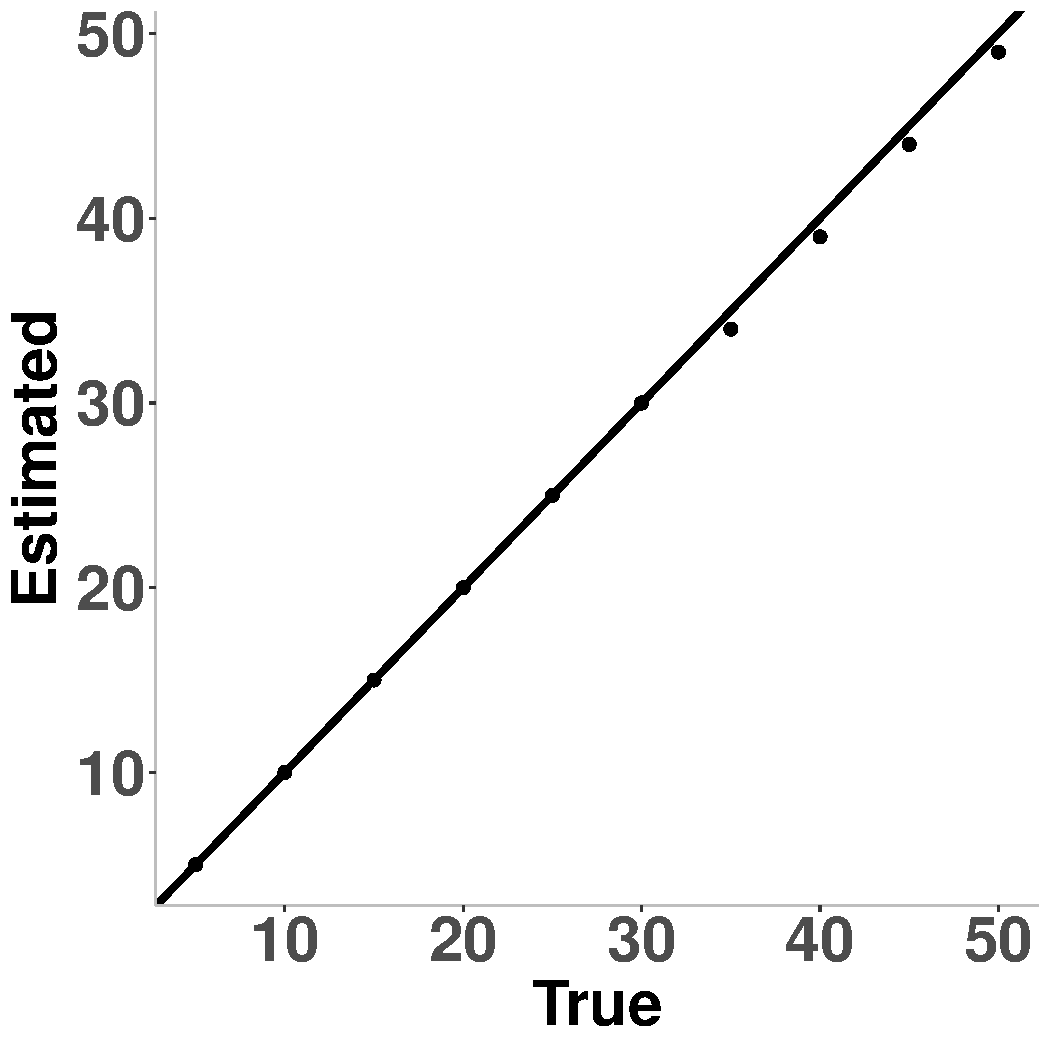
\includegraphics[width=0.3\textwidth]{PeriKResults.pdf}}
\bigskip

Parameter differences data point \tikz\draw[black,fill=black] (0,0) circle (.5ex); \;\; 1:1 line \textcolor{black}{\rule{1.5cm}{1mm}}\\

\caption{The true parameters values of $\theta$ (A), \textit{m\textsubscript{0}} (B) and \textit{K} (C) were simulated and the results fitted using the Perimeter Model analytical NLLS fitting procedure to get the parameters back. True and estimated values for the three fitted parameters are plotted above. Fittings of the Perimeter Model to simulated data returned mean R\textsuperscript{2} = 0.99, adjusted R\textsuperscript{2} = 0.99.}
\label{fig:myfig}
\end{figure}

\begin{table}[h!]
  \begin{center}
    \caption{Comparison between true and estimated mean parameters across 200 Perimeter Model simulations clustered into 10 groups where parameter values ($\theta$, \textit{m\textsubscript{0}}, \textit{K}) were the same for each simulation group with varying areas.}
    \label{table5}
    \pgfplotstabletypeset[
      multicolumn names, % allows to have multicolumn names
      col sep=comma, % the seperator in our .csv file
      display columns/0/.style={
		column name=$Parameter$, % name of first column
		string type},  % use siunitx for formatting
      display columns/1/.style={
		column name=$True$,
		column type={S},string type},
      display columns/2/.style={
		column name=$Estimated$,
		column type={S},string type},
      display columns/3/.style={
		column name=$Difference$,
		column type={S},string type},
           every head row/.style={
		before row={\toprule}, % have a rule at top
		after row={
			%\si{\ampere} & \si{\volt}\\ % the units seperated by &
			\midrule} % rule under units
			},
		every last row/.style={after row=\bottomrule}, % rule at bottom
    ]{PeriParam.csv} % filename/path to file
  \end{center}
\end{table}

\noindent The Perimeter Model fitted the simulated data well. Estimated parameters for $\theta$ were slightly higher than true parameters, whilst \textit{m\textsubscript{0}} and \textit{K} were slightly lower than the true parameters (Table 3.3). There was significant difference between the true and estimated values for $\theta$ (p=0.0002, 9 df), \textit{m\textsubscript{0}} (p=5x10\textsuperscript{5}, 9 df) and \textit{K} (p=0.04, 9df). Despite the significant difference between the estimated and true values, the differences are small and the model fitting process is considered validated and fit for applying to empirical datasets.   

\section{Model Fitting}

\subsection{Non-Linear Least Squares Fitting}


\noindent 50 of the 57 datasets exhibited a positive TAR and were used for the NLLS fitting. Of the 50 datasets 26 failed to achieve adjusted R\textsuperscript{2} scores of between 0 and 1. These datasets were excluded from further analysis (see Supplementary Materials, Figure 7.2). 

\begin{table}[h!]
  \begin{center}
    \caption{The mean R\textsuperscript{2} and adjusted R\textsuperscript{2} results for each model (Classic, Depth, Perimeter) after being successfully fitted to 24 empirical datasets.}
    \label{table5}
    \pgfplotstabletypeset[
      multicolumn names, % allows to have multicolumn names
      col sep=comma, % the seperator in our .csv file
      display columns/0/.style={
		column name=$Model$, % name of first column
		string type},  % use siunitx for formatting
      display columns/1/.style={
		column name=$R\textsuperscript{2}$,
		column type={S},string type},
      display columns/2/.style={
		column name=$Adj R\textsuperscript{2}$,
		column type={S},string type},
           every head row/.style={
		before row={\toprule}, % have a rule at top
		after row={
			%\si{\ampere} & \si{\volt}\\ % the units seperated by &
			\midrule} % rule under units
			},
		every last row/.style={after row=\bottomrule}, % rule at bottom
    ]{RResults.csv} % filename/path to file
  \end{center}
\end{table}

\noindent All three models had similar mean R\textsuperscript{2} and adjusted R\textsuperscript{2} scores and fit the data moderately well (Table 3.4). The Classic Model was best-fit for 1 dataset, Depth and Perimeter were best for 2 each and the rest of the datasets were either best described by both Classic and Depth or all of the models (Table 3.5).  \\

\begin{table}[h!]
  \begin{center}
    \caption{The best-fit models (Classic, Depth, Perimeter) by highest adjusted R\textsuperscript{2} value for each empirical dataset (note some datasets had equal adjusted R\textsuperscript{2} values for two or more models). }
    \label{table5}
    \pgfplotstabletypeset[
      multicolumn names, % allows to have multicolumn names
      col sep=comma, % the seperator in our .csv file
      display columns/0/.style={
		column name=$Models$, % name of first column
		string type},  % use siunitx for formatting
      display columns/1/.style={
		column name=$Best Fit$,
		column type={S},string type},
           every head row/.style={
		before row={\toprule}, % have a rule at top
		after row={
			%\si{\ampere} & \si{\volt}\\ % the units seperated by &
			\midrule} % rule under units
			},
		every last row/.style={after row=\bottomrule}, % rule at bottom
    ]{BestModel.csv} % filename/path to file
  \end{center}
\end{table}

\noindent The best model fits had mean R\textsuperscript{2} = 0.49 and mean adjusted R\textsuperscript{2} = 0.41 with standard deviation 0.28 and range 0.01 - 0.96. The median value of $\theta$ was 8, with a range of 0.28 -- 159709. The median value of \textit{m\textsubscript{0}} was 2.17 x10\textsuperscript{-9} with a range of 4.97 x 10\textsuperscript{-16} -- 0.56. The median value for \textit{K} was 7, with range 1 -- 424. There was no correlation between the best fitted-values of the four parameters (Table 3.6). \\

\begin{table}[h!]
  \begin{center}
    \caption{p-values of correlations between the four model parameters ($\theta$, \textit{m\textsubscript{0}}, \textit{K}, $\rho$) that show no correlation}
    \label{table5}
    \pgfplotstabletypeset[
      multicolumn names, % allows to have multicolumn names
      col sep=comma, % the seperator in our .csv file
      display columns/0/.style={
		column name=$Parameter$, % name of first column
		string type},  % use siunitx for formatting
      display columns/1/.style={
		column name=$K$,
		column type={S},string type},
      display columns/2/.style={
		column name=$Theta$,
		column type={S},string type},
        display columns/3/.style={
		column name=$m\textsubscript{0}$,
		column type={S},string type},
	 display columns/4/.style={
		column name=$rho$,
		column type={S},string type},
           every head row/.style={
		before row={\toprule}, % have a rule at top
		after row={
			%\si{\ampere} & \si{\volt}\\ % the units seperated by &
			\midrule} % rule under units
			},
		every last row/.style={after row=\bottomrule}, % rule at bottom
    ]{Spearmansrank_p_corr.csv} % filename/path to file
  \end{center}
\end{table}

%How often was the power-law model a better fit to the data than the three models?
\noindent The power-law model had the same number of successful fittings as the Classic, Depth and Perimeter models. After removing failed fits the mean \textit{z} value was 0.16. The power-law model performed more poorly than the other three models (R\textsuperscript{2}=0.47, adjusted R\textsuperscript{2}=0.38) (see Supplementary Materials, Table 7.3). AIC scores indicated that the power-law model was not a more parsimonious model than the Classic, Depth or Perimeter models relative to model fit for any of the datasets (see Supplementary Materials, Table 7.4). The Classic and Depth models were significantly better than the power-law model for 9 datasets each. The Perimeter model was a better fit than the power-law model for 5 datasets.   
  
\section{Critical Area}
{\texorpdfstring
Off the five habitat types (terrestrial, riverine, lacustrine, plant and machine) and six taxonomic groups (algae, archaea, bacteria, fungi, pathogens and protozoa), the riverine habitat and archaea group did not have any successful fittings and are excluded from the following analysis.\\


\begin{figure}[htbp]
\centering
\subfloat[Dataset 45, bacteria in biomembrane reactors]{\label{fig:a}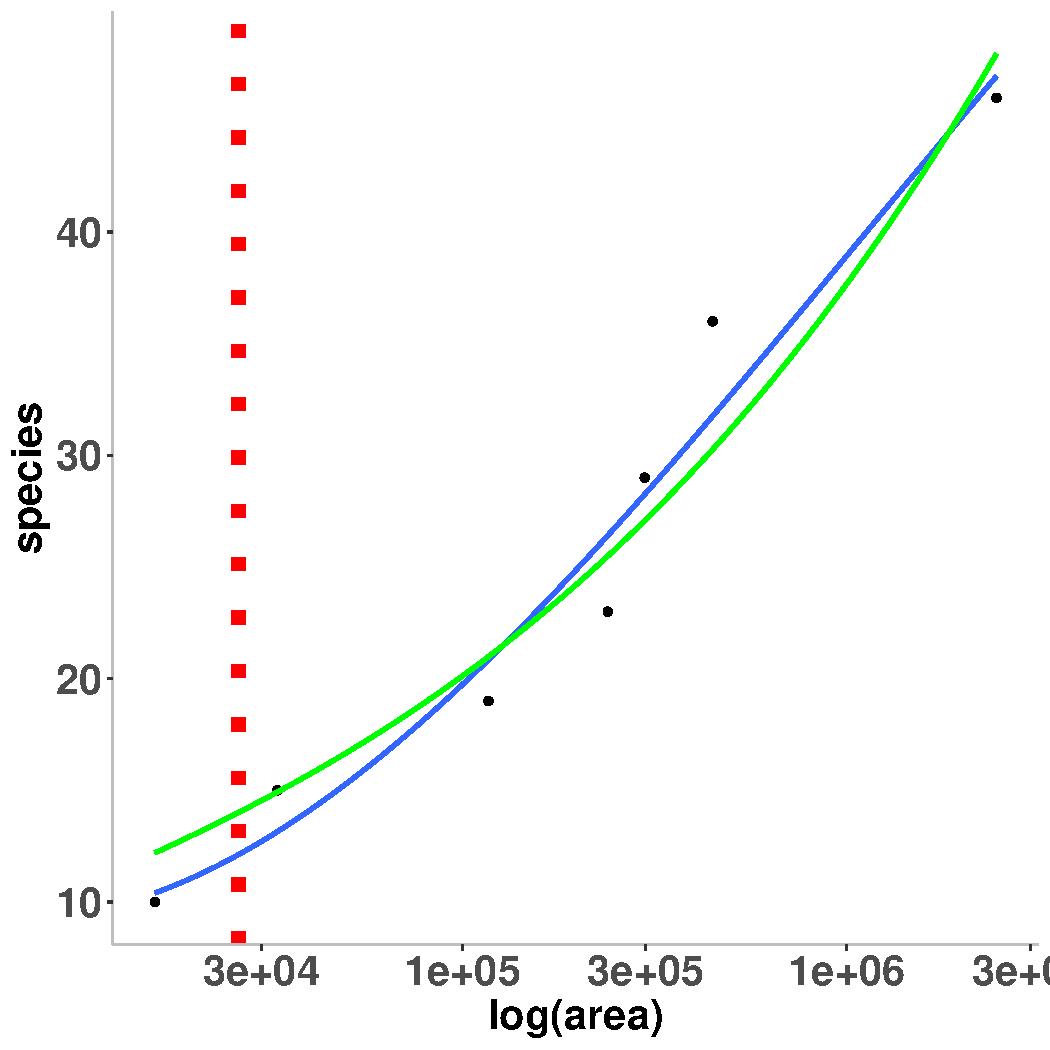
\includegraphics[width=0.45\linewidth]{../Results/ClassicNLLSPlot39.pdf}}\qquad
\subfloat[Dataset 44, fungi in plant root soil]{\label{fig:b}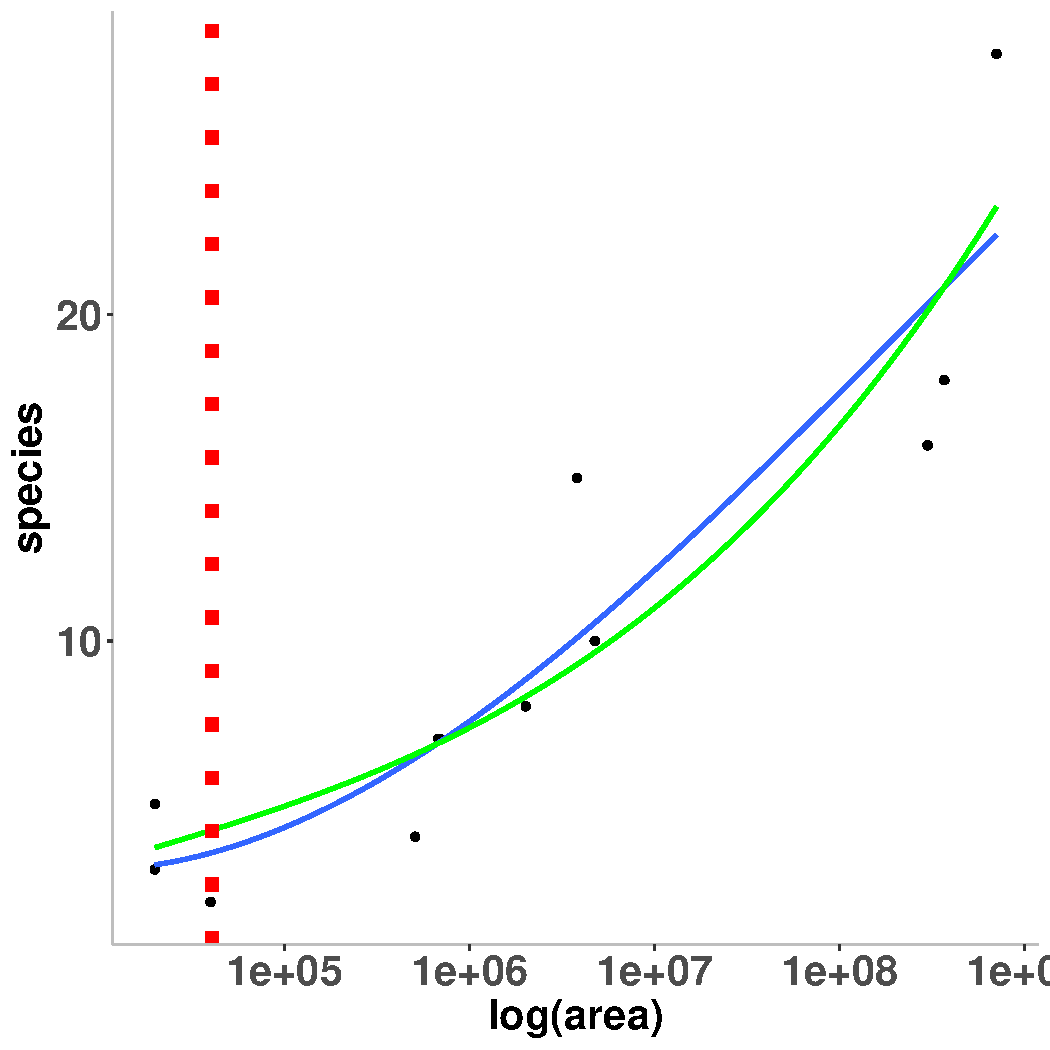
\includegraphics[width=0.45\linewidth]{../Results/PeriNLLSPlot38.pdf}}\\
\subfloat[Dataset 46, bacteria in tree holes (log area plotted with depth)]{\label{fig:c}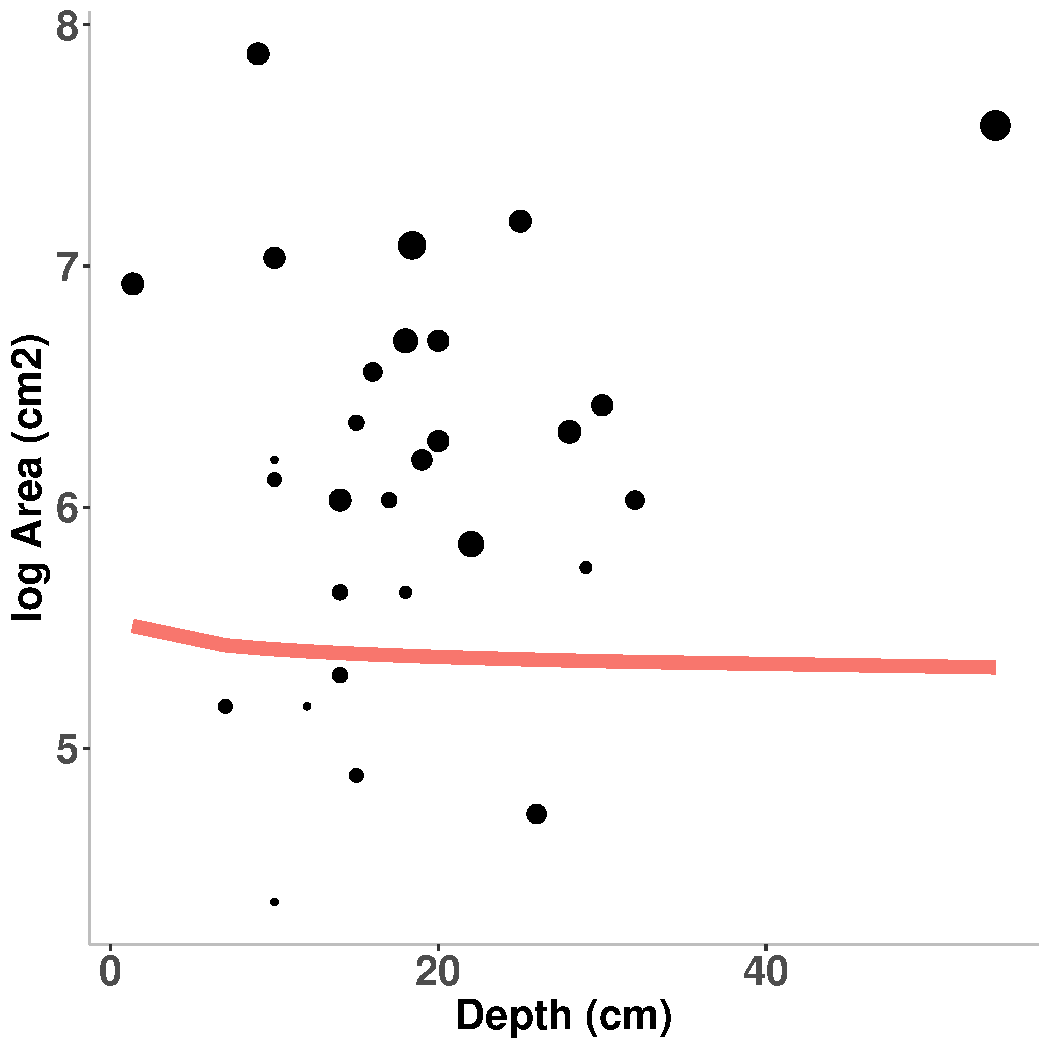
\includegraphics[width=0.45\textwidth]{../Results/DepthNLLSPlot40.pdf}}\qquad%
\subfloat[Dataset 46, bacteria in tree holes (log volume plotted with OTU richness)]{\label{fig:d}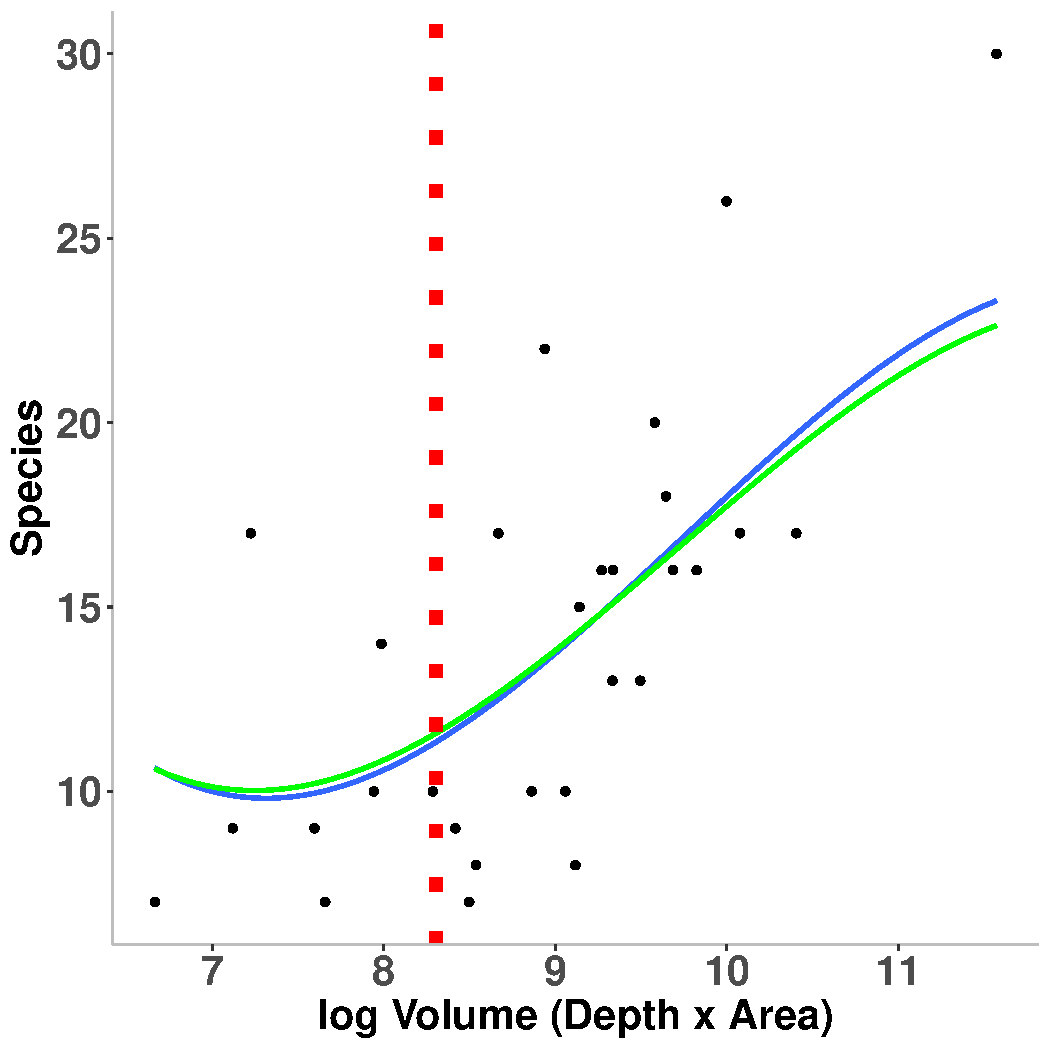
\includegraphics[width=0.45\textwidth]{../Results/DepthNLLSPlot2_40.pdf}}%
\bigskip

Simulation data point \tikz\draw[black,fill=black] (0,0) circle (.5ex); \;\;NLLS fit \textcolor{blue}{\rule{1.5cm}{1mm}} \;\;Power-Law fit \textcolor{green}{\rule{1.5cm}{1mm}}\;\; \textit{A\textsubscript{crit}/A\textsubscript{vol}}\;\; \textcolor{red}{\rule{0.1cm}{1mm}}\; \textcolor{red}{\rule{0.1cm}{1mm}}\; \textcolor{red}{\rule{0.1cm}{1mm}}\; \textcolor{red}{\rule{0.1cm}{1mm}}\\

\caption{A) Best-fit Classic Model for dataset 45, bacteria in biomembrane reactors. Red line indicates \textit{A\textsubscript{crit}}, blue line indicates NLLS fit and green line indicates power-law fit (NLLS fit: R\textsuperscript{2}=0.96, adjusted R\textsuperscript{2}=0.88, $\theta$=9, \textit{m\textsubscript{0}}=4.97 x 10\textsuperscript{-16}, \textit{K}=7, power-law fit: R\textsuperscript{2}=0.94, adjusted R\textsuperscript{2}=0.82, \textit{z}=0.27, \textit{c}=0.88). B) Best-fit Perimeter Model for dataset 44, fungi in plant soil (NLLS fit: R\textsuperscript{2}=0.85, adjusted R\textsuperscript{2}=0.77, $\theta$=5, \textit{m\textsubscript{0}}=6.15 x 10\textsuperscript{-11}, \textit{K}=2, power-law fit: R\textsuperscript{2}=0.87, adjusted R\textsuperscript{2}=0.78, \textit{z}=0.18, \textit{c}=0.64). C) Best-fit Depth Model for dataset 46, bacteria in freshwater treeholes. The size of the black circles represents increasing OTU richness at that corresponding depth (x-axis) and log area (y axis) (R\textsuperscript{2}=49, adjusted R\textsuperscript{2}=0.40, $\theta$=8, \textit{m\textsubscript{0}}=3.75 x 10\textsuperscript{-9}, \textit{K}=6, power-law fit: R\textsuperscript{2}=0.46, adjusted R\textsuperscript{2}=0.38, \textit{z}=0.33, \textit{c}=1.74). Where the red line passes through depth and area space is where \textit{A\textsubscript{crit}} occurs. D) Dataset 46 plotted as log Volume by OTU richness to illustrate the model fit and log critical volume (A\textsubscript{vol})}
\label{fig:myfig}
\end{figure}

\noindent The log \textit{A\textsubscript{crit}} data were not normally distributed with non-homogenous variances. Despite the violation of normality I have proceeded with the multiple regression analysis, although interpretation of results will take this into consideration. \\

\noindent Initial multiple regression revealed that the model was a poor fit to the data (R\textsuperscript{2}=0.39, adjusted R\textsuperscript{2}=0.05, p=0.374) and neither categorical variable was significant in predicting log \textit{A\textsubscript{crit}} (habitat type p=0.1759, taxonomic group p=0.6402). A plot of the model indicated that there was an outlying data point. After removing the outlying data point the model was significant in describing the data (R\textsuperscript{2}=0.62, adjusted R\textsuperscript{2}=0.44, p=0.02). Taxonomic group became weakly significant in predicting log \textit{A\textsubscript{crit}} (p=0.0187), habitat type did not (p=0.097). After removing habitat type as a variable the model was a similar fit to the data but more significant (R\textsuperscript{2}=0.55, adjusted R\textsuperscript{2}=0.45, p=0.004).\\

\noindent Multiple regression including taxonomic group upheld the prediction that \textit{A\textsubscript{crit}} would occur at lower areas for more motile OTUs as bacteria show the lowest log\textit{A\textsubscript{crit}} estimate and host-dependent pathogens show the highest (Table 3.7). \\

\noindent There was a large variation in mean log \textit{A\textsubscript{crit}} between habitats and taxonomic groups. Terrestrial habitats showed the highest mean log \textit{A\textsubscript{crit}} (27.33), whilst machine habitats showed the lowest (4.66) (Figure 3.6). Pathogens exhibited the largest mean log \textit{A\textsubscript{crit}} for taxonomic groups (55.15), with bacteria having the lowest (4.06) (Figure 3.6). \\

\begin{figure}[htp]

\centering
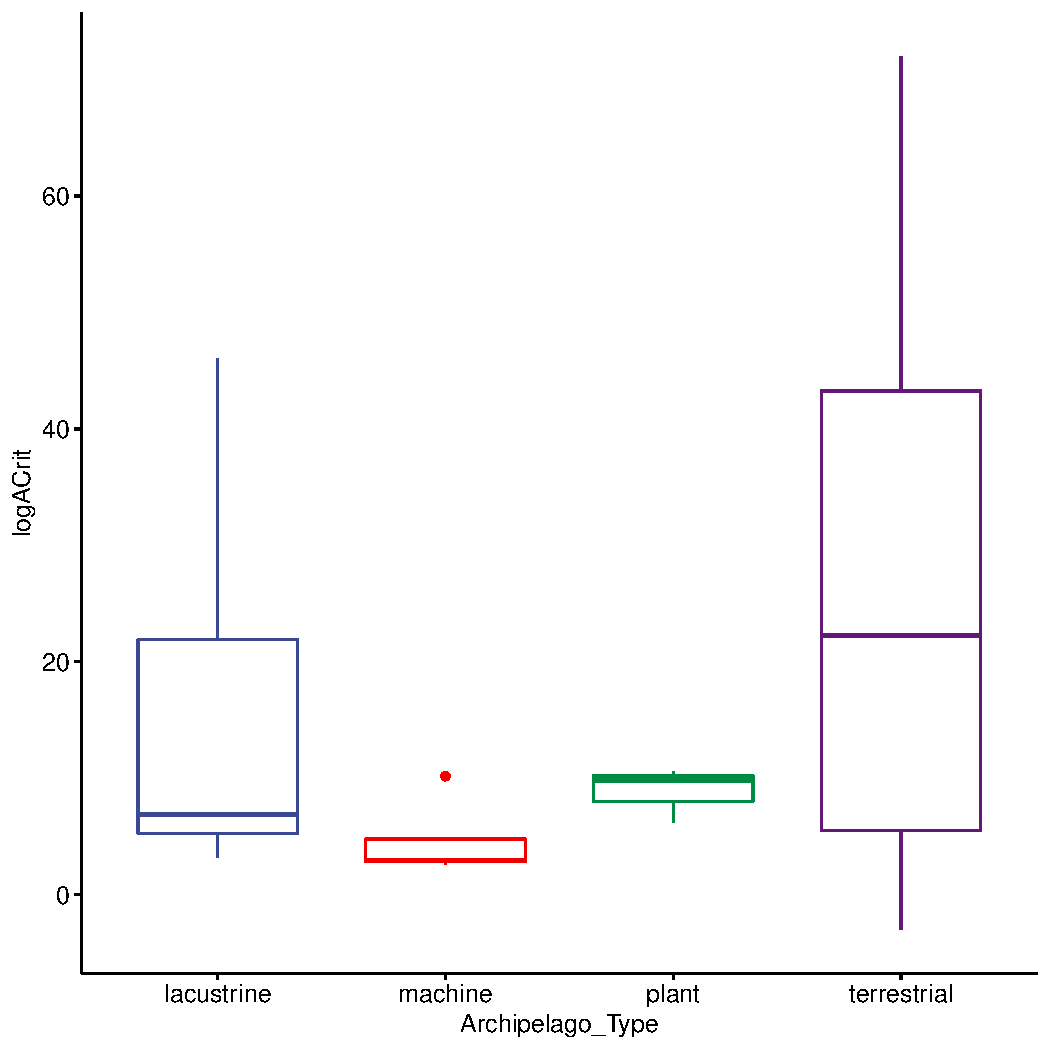
\includegraphics[width=.5\textwidth]{BoxplotTotalACritArch.pdf}\hfill
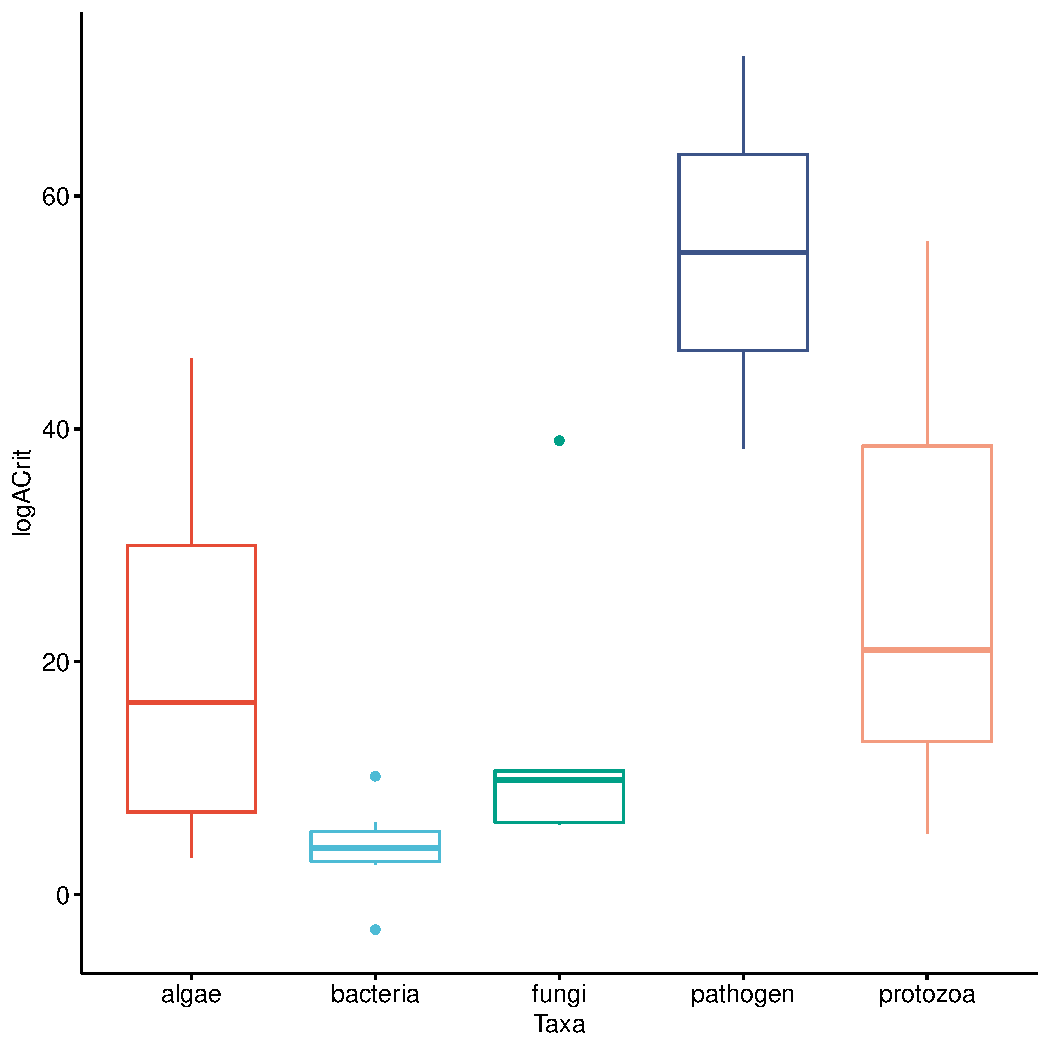
\includegraphics[width=.5\textwidth]{BoxplotTotalACritTaxa.pdf}\hfill

\hspace{10pt}\textbf{Habitat Type} \hspace{110pt} \textbf{Taxonomic Group}

\caption{log \textit{A\textsubscript{crit}} by habitat type and taxonomic group after removing anomalous result}
\label{fig:figure8}

\end{figure}


}

\begin{table}[h]
\begin{center}
    \caption{Table showing the results of multiple regression analysis of estimated effect of taxonomic group only on log \textit{A\textsubscript{crit}}}
    \label{crouch}
    \begin{tabular}{  l  p{1.5cm} p{3cm}  p{1.5cm}}
        \toprule
\textbf{Variable} 
&\textbf{Estimate}      
& \textbf{95\% CI}
& \textbf{p-value}   \\\midrule
intercept (algae)
&20.56
& [5.07, 36.07]
& 0.0121 \\\hline
taxonomic group
&
& 
&0.004 \\\hline
bacteria
&-16.500
& [-35.12, 2.12]
&0.0791 \\\hline
fungi
&-6.222 
& [-27.01, 14.56]
& 0.5373 \\\hline
pathogens
&34.587
& [7.75, 61.42]
& 0.0144 \\\hline
protozoa
&6.879 
& [-16.79, 30.55]
& 0.5491  \\
        \bottomrule
    \end{tabular}
    \end{center}
\end{table}








